\documentclass[11pt]{article}

\usepackage[review]{acl}

\usepackage{times}
\usepackage{latexsym}
\usepackage[T1]{fontenc}
\usepackage[utf8]{inputenc}
\usepackage{microtype}
\usepackage{inconsolata}
\usepackage{graphicx}

\usepackage{amsmath,amssymb}
\usepackage{booktabs}
\usepackage{multirow}
\usepackage{xcolor}
\usepackage{tikz}
\usetikzlibrary{arrows.meta,positioning,calc,shapes.geometric,decorations.pathreplacing}
\usepackage{pgfplots}
\pgfplotsset{compat=1.18}
\usepgfplotslibrary{groupplots}

% ---------- palette ----------
\definecolor{interface}{HTML}{E8730C}
\definecolor{decoder}{HTML}{3C78B4}
\definecolor{derivative}{HTML}{C0392B}
\definecolor{benign}{HTML}{4C9A5B}
\definecolor{moderate}{HTML}{E1A93A}
\definecolor{severe}{HTML}{C0392B}
\definecolor{featlow}{HTML}{A9CBEA}
\definecolor{featmid}{HTML}{5B8DC9}
\definecolor{feathigh}{HTML}{2E5A9C}

\DeclareRobustCommand*\circled[1]{\tikz[baseline=(char.base)]{\node[shape=circle,draw,inner sep=0.8pt,font=\scriptsize\bfseries] (char) {#1};}}
\newcommand{\tauacc}{\tau}
\newcommand{\Tp}{\mathcal{T}'}
\newcommand{\ours}{interface repair}
\newcommand{\Ours}{Interface repair}

\title{Mind the Interface: Repairing Speculative Drafters\\for Post-Trained Language Models}

\author{Anonymous ACL submission}

\begin{document}
\maketitle

\begin{abstract}
Speculative decoding with target-conditioned drafters such as EAGLE-3 is among the fastest ways to serve large language models, and the drafter released with a base model is routinely reused for its many fine-tuned derivatives.
We show that this reuse breaks for an important and growing class of models: derivatives produced by distilling a stronger reasoning teacher.
In a census of 174 public derivatives, quantized, merged and RL-tuned models retain 98--100\% of the family drafter's acceptance, while DeepSeek-R1-Distill-Llama-8B and Llama-3.1-Nemotron-Nano-8B lose up to 30\%, erasing most of the speedup.
We trace this loss to the drafter's \emph{feature interface}, the projection through which it reads the target's hidden states, and propose \emph{\ours{}}: re-fitting the family drafter on the derivative's own responses to public instructions, without any of the original training data.
Re-fitting the interface alone (12\% of the drafter's parameters) closes 60\% of the gap to a dedicated drafter trained specifically for the derivative, and a full warm start closes 72\%, using 11 GPU-hours, over 400$\times$ less compute than the public recipe for a dedicated drafter.
On SPEED-Bench and MATH-500, repair raises the end-to-end speedup of R1-Distill from 1.31$\times$ to 1.83$\times$ (dedicated drafter: 2.05$\times$) and of Nemotron-Nano from 1.29$\times$ to 1.80$\times$, outperforming independent draft models and training-free drafting.
\end{abstract}

% =====================================================================
\section{Introduction}
% =====================================================================

Speculative decoding has become the standard way to serve large language models (LLMs) quickly: a small drafter proposes several tokens, and the target model verifies all of them in a single forward pass, accelerating generation without changing its output \citep{leviathan2023speculative,chen2023accelerating}.
The fastest drafters today are \emph{target-conditioned}.
Rather than modeling text from scratch, they read the target's own hidden states and predict its next tokens from them \citep{cai2024medusa,li2024eagle,li2025eagle3,chen2026dflash}.
EAGLE-3, for instance, fuses features from the target's lower, middle and upper layers and reports speedups of up to 6.5$\times$ \citep{li2025eagle3}.
This tight coupling is also their price: each drafter is trained for one specific target, on hundreds of thousands of examples, for tens of epochs.

Open-weight models, however, rarely stay single models.
A popular base model such as Llama-3.1-8B-Instruct spawns thousands of derivatives on public model hubs, which are quantized, merged, aligned, RL-tuned and distilled \citep{horwitz2025atlas}.
Training a dedicated drafter for each derivative is out of reach, so serving stacks reuse the drafter released for the parent, the \emph{family drafter}, for all of its descendants \citep{kwon2023vllm,redhat2025speculators}.
Practitioners make this choice every day, yet two questions behind it remain open: when does a family drafter keep working for a derivative, and what can be done when it does not?

\begin{figure}[t]
  \centering
  % Figure 1: teaser. (a) census of family-drafter reuse; (b) speedup on R1-Distill.
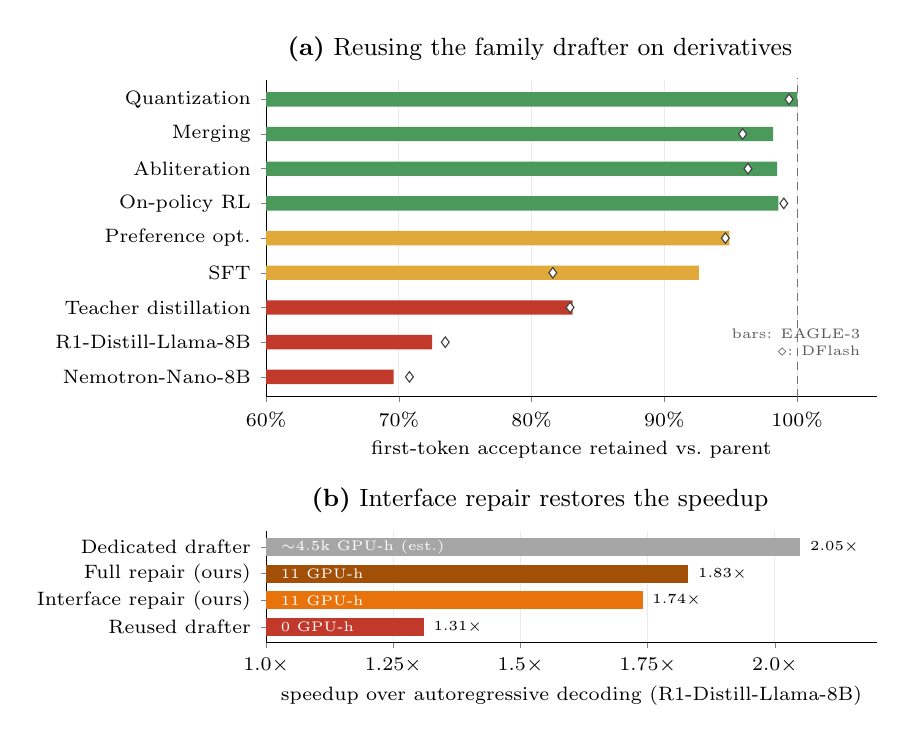
\begin{tikzpicture}
\pgfplotsset{
  teaserbar/.style={
    xbar, bar width=5.2pt, bar shift=0pt,
    width=0.77\columnwidth, height=5.6cm,
    xmin=0.6, xmax=1.06,
    symbolic y coords={Nemotron-Nano-8B,R1-Distill-Llama-8B,Teacher distillation,SFT,Preference opt.,On-policy RL,Abliteration,Merging,Quantization},
    ytick={Nemotron-Nano-8B,R1-Distill-Llama-8B,Teacher distillation,SFT,Preference opt.,On-policy RL,Abliteration,Merging,Quantization}, y dir=normal,
    yticklabel style={font=\scriptsize, align=right},
    xticklabel style={font=\scriptsize},
    xtick={0.6,0.7,0.8,0.9,1.0},
    xticklabels={60\%,70\%,80\%,90\%,100\%},
    axis x line*=bottom, axis y line*=left,
    enlarge y limits=0.07,
    tick align=outside, major tick length=2pt,
    xmajorgrids, grid style={black!8},
    clip=false,
  }
}
% ---------------- (a) census ----------------
\begin{axis}[teaserbar, name=census,
  xlabel={\scriptsize first-token acceptance retained vs.\ parent},
  xlabel style={yshift=2pt},
  title={\small\textbf{(a)} Reusing the family drafter on derivatives},
  title style={yshift=-3pt, xshift=-4mm},
]
\addplot[fill=benign, draw=none] coordinates {
  (1.000,Quantization) (0.982,Merging) (0.985,Abliteration) (0.986,On-policy RL)};
\addplot[fill=moderate, draw=none] coordinates {
  (0.949,Preference opt.) (0.926,SFT)};
\addplot[fill=severe, draw=none] coordinates {
  (0.831,Teacher distillation) (0.725,R1-Distill-Llama-8B) (0.696,Nemotron-Nano-8B)};
% DFlash markers
\addplot[only marks, mark=diamond*, mark size=1.9pt, draw=black!75, fill=white] coordinates {
  (0.994,Quantization) (0.959,Merging) (0.963,Abliteration) (0.990,On-policy RL)
  (0.946,Preference opt.) (0.816,SFT) (0.829,Teacher distillation)
  (0.735,R1-Distill-Llama-8B) (0.708,Nemotron-Nano-8B)};
\draw[densely dashed, black!55] (axis cs:1.0,{[normalized]-0.6}) -- (axis cs:1.0,{[normalized]8.6});
\node[font=\tiny, black!65, anchor=east, align=right] at (axis cs:1.055,R1-Distill-Llama-8B) {bars: EAGLE-3\\$\diamond$: DFlash};
\end{axis}
% ---------------- (b) speedup ----------------
\begin{axis}[
  at={(census.below south west)}, anchor=above north west, yshift=-0.15cm,
  xbar, bar width=6.5pt, bar shift=0pt,
  width=0.77\columnwidth, height=3.0cm,
  xmin=1.0, xmax=2.2,
  symbolic y coords={ded,full,iface,reuse},
  ytick={ded,full,iface,reuse}, y dir=reverse,
  yticklabels={Dedicated drafter,Full repair (ours),Interface repair (ours),Reused drafter},
  yticklabel style={font=\scriptsize},
  xticklabel style={font=\scriptsize},
  xtick={1.0,1.25,1.5,1.75,2.0},
  xticklabels={1.0$\times$,1.25$\times$,1.5$\times$,1.75$\times$,2.0$\times$},
  axis x line*=bottom, axis y line*=left,
  enlarge y limits=0.2, tick align=outside, major tick length=2pt,
  xmajorgrids, grid style={black!8},
  xlabel={\scriptsize speedup over autoregressive decoding (R1-Distill-Llama-8B)},
  xlabel style={yshift=2pt},
  title={\small\textbf{(b)} Interface repair restores the speedup},
  title style={yshift=-3pt, xshift=-4mm},
  clip=false,
  nodes near coords, every node near coord/.append style={font=\tiny, anchor=west},
  point meta=explicit symbolic,
]
\addplot[fill=severe, draw=none] coordinates {(1.31,reuse) [1.31$\times$]};
\addplot[fill=interface, draw=none] coordinates {(1.74,iface) [1.74$\times$]};
\addplot[fill=interface!70!black, draw=none] coordinates {(1.83,full) [1.83$\times$]};
\addplot[fill=black!35, draw=none] coordinates {(2.05,ded) [2.05$\times$]};
\node[font=\tiny, text=white, anchor=west] at (axis cs:1.01,reuse) {0 GPU-h};
\node[font=\tiny, text=white, anchor=west] at (axis cs:1.01,iface) {11 GPU-h};
\node[font=\tiny, text=white, anchor=west] at (axis cs:1.01,full) {11 GPU-h};
\node[font=\tiny, text=white, anchor=west] at (axis cs:1.01,ded) {${\sim}$4.5k GPU-h (est.)};
\end{axis}
\end{tikzpicture}

  \caption{\textbf{(a)} First-token acceptance of the Llama-3.1-8B-Instruct family drafters on public derivatives, relative to the parent model (174 derivatives grouped by post-training history; EAGLE-3 bars, DFlash diamonds). Weight-space edits and on-policy RL leave the drafter intact; distillation from a reasoning teacher breaks it. \textbf{(b)} On R1-Distill-Llama-8B, \ours{} recovers most of the speedup of a dedicated drafter at a small fraction of its training cost.}
  \label{fig:teaser}
\end{figure}

We answer the first question with a census of 174 public derivatives in the Llama-3.1-8B and Qwen3-8B families (Figure~\ref{fig:teaser}a).
For most of the ecosystem, reuse is reliable.
Quantized, merged, abliterated and on-policy RL derivatives retain 98--100\% of the family drafter's acceptance, in line with evidence that on-policy training keeps models close to their initialization \citep{shenfeld2026razor,chen2026retaining}.
Reuse fails, however, for precisely the derivatives that are most expensive to serve: models distilled from stronger reasoning teachers.
DeepSeek-R1-Distill-Llama-8B and Llama-3.1-Nemotron-Nano-8B lose 26--30\% of first-token acceptance under both EAGLE-3 and DFlash drafters.
For R1-Distill, the speedup collapses from 2.05$\times$ with a dedicated drafter to 1.31$\times$ (Figure~\ref{fig:teaser}b).
Reasoning models routinely emit thousands of tokens per query, so this lost speedup costs the most exactly where acceleration matters most.

We then show that the failure is localized.
A target-conditioned drafter accesses its target through a single learned map, the \emph{feature interface}, a dense projection that compresses the target's multi-layer hidden states into the drafter's input space.
Post-training shifts these hidden states \citep{kumar2022finetuning}, so the interface misreads them.
The rest of the drafter, namely its decoder layer and language-modeling head, encodes knowledge about drafting that transfers largely intact.
This observation suggests \emph{\ours{}} (Figure~\ref{fig:method}): elicit the derivative's own responses to public instructions, then re-fit the family drafter on them with its native training objective, updating either the interface alone or the whole warm-started drafter.
Repair needs no access to the derivative's or the drafter's training data, no new architecture, and no change to the serving engine.

\Ours{} is highly effective.
On R1-Distill-Llama-8B, re-fitting only the interface closes 60\% of the gap between the reused family drafter and a dedicated drafter trained by the EAGLE authors, and a full warm start closes 72\%.
With 11 GPU-hours of compute, over 400$\times$ less than the public recipe for a dedicated drafter, repair lifts the end-to-end speedup from 1.31$\times$ to 1.83$\times$.
On Nemotron-Nano, for which no dedicated drafter exists, it lifts the speedup from 1.29$\times$ to 1.80$\times$.
Repaired drafters are faster than training-free n-gram drafting and independent small draft models, and the gains hold across drafter checkpoints and drafter families.
In summary, we make three contributions:
\begin{itemize}
  \setlength\itemsep{1pt}
  \item We present a census of family-drafter reuse across 174 public derivatives and identify off-policy distillation as the post-training regime that breaks target-conditioned drafters (\S\ref{sec:census}).
  \item We localize the failure to the drafter's feature interface and propose \ours{}, a simple recipe that re-fits the family drafter on the derivative's own outputs without any original training data (\S\ref{sec:method}).
  \item We show on SPEED-Bench and MATH-500 that repair recovers most of a dedicated drafter's speedup at a small fraction of its cost, across targets, drafter checkpoints and drafter families (\S\ref{sec:results}).
\end{itemize}

% =====================================================================
\section{Background: Target-Conditioned Drafters}
\label{sec:background}
% =====================================================================

\paragraph{Speculative decoding.}
Given a prefix $y_{\le t}$, a drafter proposes $K$ tokens $\hat y_{t+1:t+K}$.
The target scores all of them in one forward pass and accepts the longest prefix that agrees with its own predictions, plus one bonus token that it generates itself \citep{leviathan2023speculative,chen2023accelerating}.
The output is identical to decoding with the target alone.
Efficiency is governed by the acceptance length $\tauacc$, the expected number of tokens produced per target forward pass, and by the cost of drafting.
With per-step costs $c_T$ for the target and $c_D$ for the drafter, the speedup is approximately $\tauacc \, c_T / (c_T + K c_D)$.
A good drafter is therefore both \emph{accurate} (high $\tauacc$) and \emph{cheap} (low $c_D$).

\paragraph{Target-conditioned drafting.}
Target-conditioned drafters achieve both properties by reusing the target's computation.
Medusa attaches extra decoding heads to the target's final layer \citep{cai2024medusa}, and EAGLE drafts autoregressively at the feature level \citep{li2024eagle,li2024eagle2}.
EAGLE-3 \citep{li2025eagle3} reads hidden states $h^{\text{low}}_t, h^{\text{mid}}_t, h^{\text{high}}_t \in \mathbb{R}^{d}$ from three depths of the target and maps them through a learned \emph{feature interface} $W_{\text{fc}} \in \mathbb{R}^{d \times 3d}$:
\begin{equation}
  g_t = W_{\text{fc}}\,[\,h^{\text{low}}_t ;\, h^{\text{mid}}_t ;\, h^{\text{high}}_t\,].
  \label{eq:interface}
\end{equation}
The fused feature $g_t$ is combined with the embedding of the next token and passed through a single decoder layer and a language-modeling head over a reduced draft vocabulary, producing the draft distribution $q_\theta$.
EAGLE-3 is trained with \emph{training-time test}: the drafter is unrolled on its own predictions for $k=1,\dots,k_{\max}$ steps and matched to the target's next-token distribution $p_T$ at each step,
\begin{equation}
  \mathcal{L}(\theta) = \sum_{k=1}^{k_{\max}} \mathbb{E}_{t}\, \mathrm{KL}\!\left(p_{T}(\cdot \mid y_{\le t+k}) \,\big\|\, q^{(k)}_\theta\right),
  \label{eq:ttt}
\end{equation}
so that it learns to draft from its own predictions as it does at inference.
DFlash \citep{chen2026dflash} drafts an entire block in parallel with a lightweight diffusion model, but it reads the target through the same kind of multi-layer feature projection.

\paragraph{Family drafters.}
A drafter is trained once for a base model and released publicly.
Serving engines then load it for any model that shares that base model's architecture and tokenizer \citep{kwon2023vllm,redhat2025speculators}.
We call the base model the \emph{parent} $T$, its drafter the \emph{family drafter} $D_{\theta_0}$, and the model being served the \emph{derivative} $\Tp$.

% =====================================================================
\section{When Family Drafters Fail}
\label{sec:census}
% =====================================================================

\paragraph{A census of derivatives.}
We collect 174 public derivatives in the Llama-3.1-8B and Qwen3-8B families \citep{llama3herd,qwen3} from the Hugging Face hub, all of which load with the architecture and tokenizer of the instruction-tuned parent and its released drafters.
We label each by its post-training history as described in its model card: quantization, merging, abliteration, supervised fine-tuning (SFT), preference optimization, on-policy reinforcement learning, or distillation from a teacher.
For every derivative, we serve the family EAGLE-3 and DFlash drafters with vLLM \citep{kwon2023vllm} and measure \emph{first-token acceptance}, the probability that the target accepts the drafter's first proposed token, on identical prompts for the derivative and its parent.
We report retention, the derivative's acceptance divided by the parent's.
First-token acceptance is independent of response length, which itself changes with post-training, and so isolates how well the drafter predicts the derivative.

\paragraph{Distillation breaks the drafter.}
Figure~\ref{fig:teaser}a shows a clear ordering.
Edits in weight space leave the drafter intact: quantized derivatives retain 100\% of the parent's acceptance, merged ones 98\% and abliterated ones 99\%.
On-policy RL does not disturb it either (99\%).
Off-policy supervision erodes acceptance progressively, from 95\% for preference optimization and 93\% for SFT to 83\% for distillation from a teacher.
The most severe losses occur for the two widely used reasoning distills.
R1-Distill-Llama-8B, trained on the outputs of DeepSeek-R1 \citep{deepseek2025r1}, retains 72.5\% under EAGLE-3 and 73.5\% under DFlash.
Nemotron-Nano-8B \citep{bercovich2025nemotron} retains 69.6\% and 70.8\%.
This ordering mirrors how far each regime moves a model from its initialization.
On-policy RL learns from the model's own samples and stays close to it \citep{shenfeld2026razor,chen2026retaining}, whereas distillation fits the model to a different model's distribution \citep{hinton2015distilling,kim2016sequence} and reshapes its internal representations.

The cost of this loss is substantial.
On R1-Distill, the reused drafter reaches an acceptance length of only 1.76 tokens per step on SPEED-Bench, compared with 2.85 for a dedicated EAGLE-3 drafter that the EAGLE authors trained on R1-Distill.
In end-to-end decoding, this is the difference between 1.31$\times$ and 2.05$\times$ (\S\ref{sec:results}).
A dedicated drafter is rarely an option: the public EAGLE-3 recipe trains on more than half a million examples for tens of epochs, and for most derivatives, including Nemotron-Nano, no dedicated drafter exists at all.
Practitioners can, however, tell cheaply when reuse is at risk.
Measuring acceptance on just 16 requests identifies the degraded derivatives in our census with an AUROC of 0.91 for EAGLE-3 and 0.93 for DFlash.

\paragraph{The failure lies in the interface.}
To find which part of the drafter breaks, we re-fit individual components of the R1-Distill family drafter on 256 of the derivative's responses (\S\ref{sec:method}) and measure how much of the gap to the dedicated drafter each closes (Table~\ref{tab:components}).
Adapting the decoder layer with LoRA \citep{hu2022lora} closes only 10\% of the gap, and recalibrating the statistics of the target's features closes none.
Re-fitting the dense feature interface closes 36\%, nearly as much as updating the interface and decoder together (37\%) and most of what fine-tuning the entire drafter achieves (46\%).
Low-rank updates of the interface fall well short (5--15\%).
This pattern indicates that post-training does not perturb the derivative's features slightly but requires a full re-mapping of how they should be read.
The drafter's decoder and head remain good at drafting.
What fails is the interface, which no longer understands the features of the model it serves.

\begin{table}[t]
  \centering
  \small
  \setlength{\tabcolsep}{5pt}
  \begin{tabular}{@{}lrr@{}}
    \toprule
    Re-fitted component & Params & Gap closed \\
    \midrule
    none (reuse) & 0 & 0\% \\
    feature statistics (affine) & 25K & 0\% \\
    decoder layer (LoRA) & 1.2M & 10\% \\
    interface, rank 8 & 0.13M & 5\% \\
    interface, rank 32 & 0.52M & 15\% \\
    \textbf{interface, dense} & 50M & \textbf{36\%} \\
    interface + decoder (LoRA) & 52M & 37\% \\
    entire drafter & 425M & 46\% \\
    \bottomrule
  \end{tabular}
  \caption{Which component should be re-fitted? Fraction of the acceptance-length gap between the reused family drafter and a dedicated drafter that each re-fit closes on R1-Distill-Llama-8B (SPEED-Bench, 256 repair examples). The dense feature interface alone accounts for most of the recoverable gain.}
  \label{tab:components}
\end{table}

% =====================================================================
\section{Interface Repair}
\label{sec:method}
% =====================================================================

\begin{figure*}[t]
  \centering
  \resizebox{\textwidth}{!}{% Figure 2: method overview (hero figure).
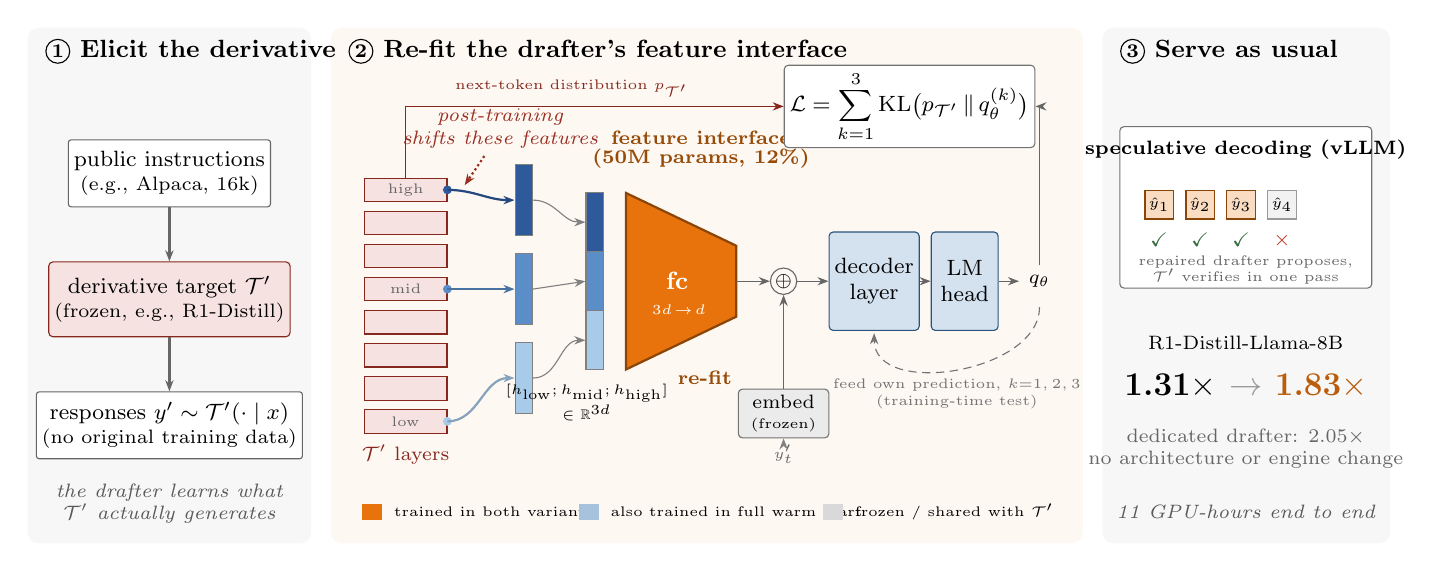
\begin{tikzpicture}[
  font=\footnotesize,
  >={Stealth[length=4pt]},
  doc/.style={draw=black!60, fill=white, rounded corners=1pt, minimum width=2.5cm, minimum height=0.85cm, align=center, inner sep=2pt},
  blk/.style={draw=black!55, rounded corners=1.5pt, align=center, inner sep=2pt},
  layer/.style={draw=derivative!70!black, fill=derivative!14, minimum width=1.05cm, minimum height=0.30cm, inner sep=0pt},
  hdr/.style={font=\small\bfseries, anchor=west},
  feat/.style={draw=black!50, minimum width=0.22cm, minimum height=0.9cm, inner sep=0pt},
  note/.style={font=\scriptsize\itshape, text=black!65, align=center},
]
% ===================== panel backgrounds =====================
\fill[black!3, rounded corners=4pt] (-0.25,-1.55) rectangle (3.35,5.0);
\fill[interface!5, rounded corners=4pt] (3.6,-1.55) rectangle (13.15,5.0);
\fill[black!3, rounded corners=4pt] (13.4,-1.55) rectangle (17.05,5.0);
\node[hdr] at (-0.15,4.7) {\circled{1} Elicit the derivative};
\node[hdr] at (3.7,4.7) {\circled{2} Re-fit the drafter's feature interface};
\node[hdr] at (13.5,4.7) {\circled{3} Serve as usual};

% ===================== (1) elicit =====================
\node[doc] (prompts) at (1.55,3.15) {public instructions\\[-1pt]\scriptsize(e.g., Alpaca, 16k)};
\node[blk, fill=derivative!14, draw=derivative!70!black, minimum width=2.5cm, minimum height=0.95cm] (tgt) at (1.55,1.55) {derivative target $\mathcal{T}'$\\[-1pt]\scriptsize(frozen, e.g., R1-Distill)};
\node[doc] (resp) at (1.55,-0.05) {responses $y' \sim \mathcal{T}'(\cdot \mid x)$\\[-1pt]\scriptsize(no original training data)};
\draw[->, thick, black!60] (prompts) -- (tgt);
\draw[->, thick, black!60] (tgt) -- (resp);
\node[note] at (1.55,-1.05) {the drafter learns what\\$\mathcal{T}'$ actually generates};

% ===================== (2) re-fit =====================
% target stack
\foreach \i in {0,...,7} {
  \node[layer] (L\i) at (4.55,0.0+0.42*\i) {};
}
\node[font=\scriptsize, text=derivative!70!black] at (4.55,-0.42) {$\mathcal{T}'$ layers};
\node[font=\tiny, text=black!60] at (4.55,0.0) {low};
\node[font=\tiny, text=black!60] at (4.55,1.68) {mid};
\node[font=\tiny, text=black!60] at (4.55,2.94) {high};
% taps
\coordinate (tapL) at (5.08,0.0);
\coordinate (tapM) at (5.08,1.68);
\coordinate (tapH) at (5.08,2.94);
\foreach \t/\c in {tapL/featlow, tapM/featmid, tapH/feathigh} { \fill[\c] (\t) circle (1.6pt); }
% feature vectors
\node[feat, fill=featlow] (fl) at (6.05,0.55) {};
\node[feat, fill=featmid] (fm) at (6.05,1.68) {};
\node[feat, fill=feathigh] (fh) at (6.05,2.81) {};
\draw[->, featlow!80!black, thick] (tapL) to[out=0,in=180] (fl.west);
\draw[->, featmid!80!black, thick] (tapM) -- (fm.west);
\draw[->, feathigh!80!black, thick] (tapH) to[out=0,in=180] (fh.west);
% concat vector
\node[feat, minimum height=0.75cm, fill=featlow]  (c1) at (6.95,1.03) {};
\node[feat, minimum height=0.75cm, fill=featmid]  (c2) at (6.95,1.78) {};
\node[feat, minimum height=0.75cm, fill=feathigh] (c3) at (6.95,2.53) {};
\draw[->, black!50] (fl.east) to[out=0,in=180] (c1.west);
\draw[->, black!50] (fm.east) -- (c2.west);
\draw[->, black!50] (fh.east) to[out=0,in=180] (c3.west);
\node[font=\tiny, align=center, anchor=north] at (6.85,0.6) {$[h_{\text{low}};h_{\text{mid}};h_{\text{high}}]$\\$\in\mathbb{R}^{3d}$};
% shift annotation
\node[note, text=derivative!80!black, anchor=south] at (5.75,3.35) {post-training\\shifts these features};
\draw[->, derivative!80!black, densely dotted, thick] (5.55,3.37) -- (5.3,3.0);
% interface trapezoid
\fill[interface, draw=interface!60!black, thick] (7.35,0.66) -- (8.75,1.33) -- (8.75,2.23) -- (7.35,2.9) -- cycle;
\node[font=\small\bfseries, text=white] at (8.0,1.78) {fc};
\node[font=\tiny, text=white] at (8.02,1.42) {$3d\!\to\!d$};
\node[font=\scriptsize\bfseries, text=interface!65!black, align=center] at (8.3,3.45) {feature interface\\[-1pt]\scriptsize(50M params, 12\%)};
\node[font=\scriptsize, text=interface!65!black, align=center] at (8.35,0.55) {\textbf{re-fit}};
% token embedding
\node[blk, fill=black!8, minimum width=1.15cm, minimum height=0.5cm] (emb) at (9.35,0.1) {\scriptsize embed\\[-2pt]\tiny(frozen)};
\node[circle, draw=black!60, inner sep=0.5pt, font=\scriptsize] (plus) at (9.35,1.78) {$\oplus$};
\draw[->, black!60] (8.75,1.78) -- (plus.west);
\draw[->, black!60] (emb.north) -- (plus.south);
\node[font=\tiny, text=black!60] at (9.35,-0.42) {$y'_{t}$};
\draw[->, black!50] (9.35,-0.3) -- (emb.south);
% decoder + head
\node[blk, fill=decoder!22, draw=decoder!70!black, minimum width=1.05cm, minimum height=1.25cm] (dec) at (10.5,1.78) {decoder\\layer};
\node[blk, fill=decoder!22, draw=decoder!70!black, minimum width=0.85cm, minimum height=1.25cm] (head) at (11.65,1.78) {LM\\head};
\draw[->, black!60] (plus.east) -- (dec.west);
\draw[->, black!60] (dec.east) -- (head.west);
\node[font=\scriptsize] (q) at (12.6,1.78) {$q_\theta$};
\draw[->, black!60] (head.east) -- (q.west);
% TTT loop
\draw[->, black!55, densely dashed] (12.6,1.45) to[out=-90,in=-90, looseness=1.0] node[pos=0.5, below, font=\tiny, align=center] {feed own prediction, $k{=}1,2,3$\\(training-time test)} (10.5,1.12);
% loss
\node[blk, fill=white, minimum height=0.55cm] (loss) at (10.95,4.0) {$\displaystyle \mathcal{L}=\sum_{k=1}^{3}\mathrm{KL}\big(p_{\mathcal{T}'}\,\|\,q^{(k)}_\theta\big)$};
\draw[->, derivative!70!black] (L7.north) |- node[pos=0.72, above, font=\tiny] {next-token distribution $p_{\mathcal{T}'}$} (loss.west);
\draw[->, black!60] (q.north) |- (loss.east);
% legend
\fill[interface] (4.0,-1.25) rectangle (4.25,-1.05); \node[font=\tiny, anchor=west] at (4.28,-1.15) {trained in both variants};
\fill[decoder!45] (6.75,-1.25) rectangle (7.0,-1.05); \node[font=\tiny, anchor=west] at (7.03,-1.15) {also trained in full warm start};
\fill[black!15] (9.85,-1.25) rectangle (10.1,-1.05); \node[font=\tiny, anchor=west] at (10.13,-1.15) {frozen / shared with $\mathcal{T}'$};

% ===================== (3) serve =====================
\node[blk, fill=white, minimum width=3.2cm, minimum height=2.05cm, anchor=north] (srv) at (15.22,3.75) {};
\node[font=\scriptsize\bfseries, anchor=north] at (15.22,3.7) {speculative decoding (vLLM)};
% draft tokens
\foreach \j/\ok in {0/1,1/1,2/1,3/0} {
  \pgfmathsetmacro{\xx}{14.12+0.52*\j}
  \ifnum\ok=1
    \node[draw=interface!60!black, fill=interface!25, minimum size=0.36cm, inner sep=0pt, font=\tiny] at (\xx,2.75) {$\hat y_{\the\numexpr\j+1\relax}$};
    \node[font=\scriptsize, text=benign!70!black] at (\xx,2.3) {\checkmark};
  \else
    \node[draw=black!40, fill=black!5, minimum size=0.36cm, inner sep=0pt, font=\tiny] at (\xx,2.75) {$\hat y_{\the\numexpr\j+1\relax}$};
    \node[font=\scriptsize, text=severe] at (\xx,2.3) {$\times$};
  \fi
}
\node[font=\tiny, text=black!60, align=center] at (15.22,1.92) {repaired drafter proposes,\\$\mathcal{T}'$ verifies in one pass};
\node[font=\scriptsize, align=center] at (15.22,1.0) {R1-Distill-Llama-8B};
\node[font=\large\bfseries, align=center] at (15.22,0.45) {1.31$\times$ \textcolor{black!40}{$\rightarrow$} \textcolor{interface!80!black}{1.83$\times$}};
\node[font=\scriptsize, text=black!60, align=center] at (15.22,-0.35) {dedicated drafter: 2.05$\times$\\no architecture or engine change};
\node[note] at (15.22,-1.15) {11 GPU-hours end to end};
\end{tikzpicture}
}
  \caption{\textbf{\Ours{}.} \circled{1} The derivative target $\Tp$ answers public instructions, producing data that reflect what it actually generates; none of its training data, nor the drafter's, is needed. \circled{2} A teacher-forced pass of $\Tp$ exposes the multi-layer hidden states that the drafter reads and the next-token distribution it must match. Post-training has shifted these features, so we re-fit the drafter's feature interface (orange) with its native training-time-test objective, optionally warm-starting the decoder layer and head as well (blue). \circled{3} The repaired drafter keeps its architecture and format, so it is served with an unchanged engine.}
  \label{fig:method}
\end{figure*}

Given a derivative $\Tp$ and the family drafter $D_{\theta_0}$ of its parent, \ours{} produces a drafter $D_{\theta}$ that is matched to $\Tp$.
It does so without the data used to train either model.
The recipe has three steps (Figure~\ref{fig:method}).

\paragraph{Eliciting the derivative.}
The drafter must predict what $\Tp$ will generate, so we let $\Tp$ show it.
We sample instructions $x$ from a public instruction corpus.
We use 16k instructions from Alpaca \citep{taori2023alpaca}, deduplicated against all evaluation prompts.
We render each instruction with the derivative's chat template and greedily decode a response $y' \sim \Tp(\cdot \mid x)$ of up to 512 tokens.
For a reasoning distill, these responses are long reasoning traces, exactly the text the drafter will face in deployment.
This mirrors sequence-level distillation \citep{kim2016sequence} and drafter alignment \citep{zhou2024distillspec,goel2024direct}, with one difference: only the drafter learns, and only to follow a fixed target.

\paragraph{Re-fitting the drafter.}
For each pair $(x, y')$, a single teacher-forced pass of $\Tp$ provides, at every response position, the three hidden states that enter Eq.~\eqref{eq:interface} and the next-token distribution $p_{\Tp}$.
We minimize the drafter's native training-time-test objective (Eq.~\ref{eq:ttt}) with $p_{\Tp}$ in place of $p_T$ and $k_{\max} = 3$, starting from the family drafter's parameters $\theta_0$.
We consider two operating points:
\begin{itemize}
  \setlength\itemsep{1pt}
  \item \textbf{Interface repair} updates only $W_{\text{fc}}$, 50M parameters or 12\% of the drafter, and keeps the decoder layer and head frozen.
  \item \textbf{Full repair} warm-starts all drafter parameters from $\theta_0$; the token embedding remains shared with $\Tp$.
\end{itemize}
Both variants inherit everything the family drafter already knows about drafting and only teach it to read the new target.
This warm start is essential.
The same architecture trained from scratch on the same data and budget falls below even the reused drafter (\S\ref{sec:results}).

\paragraph{Cost and deployment.}
Repair takes one pass over 16k examples, or 7.9M response tokens.
Generating the responses and training together take about 11 A40 GPU-hours.
The repaired drafter has the same architecture, vocabulary and file format as the family drafter, so it is a drop-in replacement in the serving engine.

% =====================================================================
\section{Experimental Setup}
\label{sec:setup}
% =====================================================================

\paragraph{Targets and drafters.}
We study the two reasoning distills from the census: DeepSeek-R1-Distill-Llama-8B, distilled from DeepSeek-R1 into Llama-3.1-8B \citep{deepseek2025r1}, and Llama-3.1-Nemotron-Nano-8B-v1, derived from Llama-3.1-8B-Instruct through distillation and reasoning post-training \citep{bercovich2025nemotron}.
Both share the Llama-3.1 architecture and tokenizer, and hence the family drafters of Llama-3.1-8B-Instruct.
Our main family drafter is the EAGLE-3 drafter that the EAGLE authors released for Llama-3.1-8B-Instruct \citep{li2025eagle3}.
We also repair the production EAGLE-3 drafter distributed with vLLM's speculators library \citep{redhat2025speculators} and the DFlash drafter \citep{chen2026dflash}.
As an upper reference, we use the dedicated EAGLE-3 drafter that the EAGLE authors trained specifically for R1-Distill-Llama-8B.

\paragraph{Baselines.}
We compare against
(i) reusing the family drafter unchanged;
(ii) n-gram prompt lookup \citep{saxena2023pld}, a training-free drafter built into vLLM;
(iii) an independent draft model, Llama-3.2-1B-Instruct \citep{llama3herd}, which shares the targets' tokenizer; and
(iv) training the same EAGLE-3 architecture from scratch on our repair data with the same budget.
All speculative methods propose $K{=}4$ tokens per step.

\paragraph{Benchmarks and metrics.}
We evaluate on SPEED-Bench \citep{abramovich2026speedbench}, a unified benchmark for speculative decoding, using a stratified 128-prompt sample of its qualitative split, which spans eleven domains from coding and math to writing, roleplay and multilingual chat.
For long-form reasoning, we use MATH-500 \citep{hendrycks2021math,lightman2024verify}.
Prompts are rendered with each target's chat template, and responses are generated greedily for up to 512 tokens.
We report the acceptance length $\tauacc$ (including the bonus token) and, for R1-Distill, the \emph{gap closed}, $(\tauacc_{\text{repair}} - \tauacc_{\text{reuse}}) / (\tauacc_{\text{dedicated}} - \tauacc_{\text{reuse}})$.
We also measure end-to-end wall-clock speedup over autoregressive decoding in vLLM on NVIDIA A40 GPUs at batch sizes 1 and 8.
Main R1-Distill results on SPEED-Bench average three training seeds, whose gap closed varies by at most 2.5 points.
Further details are in Appendix~\ref{app:details}.

% =====================================================================
\section{Results}
\label{sec:results}
% =====================================================================

\begin{table*}[t]
  \centering
  \small
  \setlength{\tabcolsep}{4.6pt}
  \begin{tabular}{@{}l c cccc c cccc@{}}
    \toprule
    & & \multicolumn{4}{c}{\textbf{R1-Distill-Llama-8B}} & & \multicolumn{4}{c}{\textbf{Nemotron-Nano-8B}} \\
    \cmidrule(lr){3-6} \cmidrule(lr){8-11}
    & Training & \multicolumn{2}{c}{$\tauacc$ $\uparrow$} & \multicolumn{2}{c}{Speedup $\uparrow$} & & \multicolumn{2}{c}{$\tauacc$ $\uparrow$} & \multicolumn{2}{c}{Speedup $\uparrow$} \\
    \cmidrule(lr){3-4} \cmidrule(lr){5-6} \cmidrule(lr){8-9} \cmidrule(lr){10-11}
    Method & GPU-h & SPEED & MATH & bs\,1 & bs\,8 & & SPEED & MATH & bs\,1 & bs\,8 \\
    \midrule
    Autoregressive decoding & -- & 1.00 & 1.00 & 1.00$\times$ & 1.00$\times$ & & 1.00 & 1.00 & 1.00$\times$ & 1.00$\times$ \\
    N-gram prompt lookup & -- & 1.49 & 1.59 & -- & -- & & 1.56 & 1.49 & -- & -- \\ % TODO: n-gram timing; MATH values are the 64-problem subset
    Independent drafter (Llama-3.2-1B) & -- & 2.44 & 2.97 & 1.26$\times$ & 1.11$\times$ & & 2.65 & 2.84 & 1.37$\times$ & 1.24$\times$ \\ % TODO: Nemotron MATH = 64-problem subset
    Family drafter, reused & 0 & 1.76 & 1.93 & 1.31$\times$ & 1.07$\times$ & & 1.76 & 1.70 & 1.29$\times$ & 1.13$\times$ \\
    Family architecture, from scratch & 11 & 1.52 & 1.67 & -- & -- & & -- & -- & -- & -- \\ % TODO: scratch MATH = 64-problem subset; Nemotron scratch not run
    \midrule
    \textbf{Interface repair (ours)} & 11 & 2.41 & 2.77 & 1.74$\times$ & 1.27$\times$ & & 2.42 & 2.72 & 1.69$\times$ & 1.39$\times$ \\
    \textbf{Full repair (ours)} & 11 & \textbf{2.54} & \textbf{2.97} & \textbf{1.83$\times$} & \textbf{1.29$\times$} & & 2.49 & \textbf{2.91} & \textbf{1.80$\times$} & \textbf{1.42$\times$} \\ % TODO: Nemotron MATH = 64-problem subset
    \midrule
    \textcolor{black!60}{Dedicated drafter (reference)} & \textcolor{black!60}{${\sim}$4.5k} & \textcolor{black!60}{2.85} & \textcolor{black!60}{3.84} & \textcolor{black!60}{2.05$\times$} & \textcolor{black!60}{1.41$\times$} & & \multicolumn{4}{c}{\textcolor{black!60}{\emph{not available}}} \\
    \bottomrule
  \end{tabular}
  \caption{\textbf{Main results.} Acceptance length $\tauacc$ on SPEED-Bench and MATH-500 and end-to-end speedup over autoregressive decoding (vLLM, A40, batch sizes 1 and 8). Repairing the family drafter recovers most of a dedicated drafter's speedup and is the fastest method that does not require a per-derivative drafter trained from scratch. Training cost includes generating the repair data; the dedicated drafter's cost is estimated for the public EAGLE-3 recipe.}
  \label{tab:main}
\end{table*}

\subsection{Main Results}

Table~\ref{tab:main} summarizes our results.
On R1-Distill-Llama-8B, full repair raises the acceptance length from 1.76 to 2.54 on SPEED-Bench and from 1.93 to 2.97 on MATH-500, closing 72\% and 54\% of the gap to the dedicated drafter.
\Ours{} alone closes 60\% and 44\% while updating only 12\% of the parameters.
These gains carry over to wall-clock time.
At batch size 1, the repaired drafters accelerate decoding by 1.83$\times$ and 1.74$\times$, against 1.31$\times$ for the reused drafter and 2.05$\times$ for the dedicated one.
In other words, full repair delivers 79\% of the dedicated drafter's acceleration over autoregressive decoding for an estimated 0.25\% of its training compute.
On Nemotron-Nano, where no dedicated drafter exists and repair is the only way to obtain a matched drafter, the speedup rises from 1.29$\times$ to 1.80$\times$.
The improvements persist under batching, where speculative decoding has less idle compute to exploit: at batch size 8, repair lifts the speedup from 1.07$\times$ to 1.29$\times$ on R1-Distill and from 1.13$\times$ to 1.42$\times$ on Nemotron-Nano.

\paragraph{The family drafter is the asset.}
Training the same EAGLE-3 architecture from scratch on the repair data reaches an acceptance length of only 1.52 on SPEED-Bench, below even the unrepaired family drafter.
A drafter's ability to draft is expensive to acquire and is exactly what the family drafter already has.
Repair preserves this ability and spends its budget on the one component that is out of date.

\paragraph{Repair versus other drafters.}
Training-free n-gram lookup rarely finds long matches in open-ended generation and stays below 1.6 tokens per step.
The independent Llama-3.2-1B drafter predicts the derivatives well, since it is itself a capable language model, but it must run sixteen transformer layers for every drafted token.
Its drafting cost consumes most of its acceptance advantage, and it reaches only 1.26$\times$ on R1-Distill and 1.37$\times$ on Nemotron-Nano.
Repaired drafters combine high acceptance with the near-free drafting of a single-layer, target-conditioned head and are therefore the fastest option on both targets and at both batch sizes.

\begin{figure*}[t]
  \centering
  % Figure 3: (a) gap closed vs. repair data; (b) speedup vs. training compute.
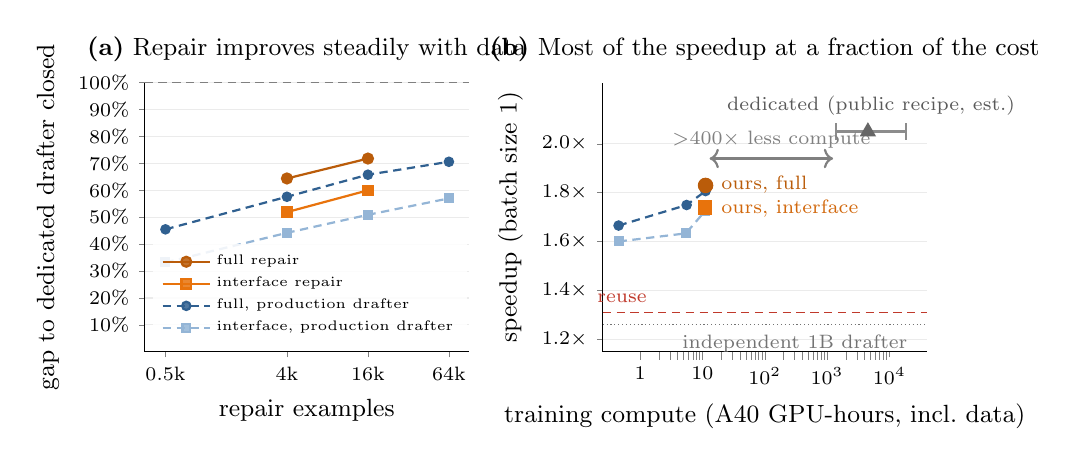
\begin{tikzpicture}
\begin{groupplot}[
  group style={group size=2 by 1, horizontal sep=1.7cm},
  width=0.47\textwidth, height=5.0cm,
  tick label style={font=\scriptsize},
  label style={font=\small},
  title style={font=\small, yshift=-2pt},
  axis x line*=bottom, axis y line*=left,
  tick align=outside, major tick length=2pt,
  grid style={black!8}, ymajorgrids,
  legend style={font=\scriptsize, draw=none, fill=white, fill opacity=0.85, text opacity=1, cells={anchor=west}, row sep=-1pt},
]
% ---------------- (a) data scaling ----------------
\nextgroupplot[
  xmode=log, log basis x=2,
  xmin=0.35, xmax=90,
  xtick={0.5,4,16,64}, xticklabels={0.5k,4k,16k,64k},
  ymin=0, ymax=100,
  ytick={10,20,30,40,50,60,70,80,90,100},
  yticklabel={\pgfmathprintnumber{\tick}\%},
  xlabel={repair examples},
  ylabel={gap to dedicated drafter closed},
  title={\textbf{(a)} Repair improves steadily with data},
  legend style={at={(axis cs:88,2)}, anchor=south east, font=\tiny},
]
\draw[densely dashed, black!50] (axis cs:0.35,100) -- (axis cs:90,100);
\node[font=\scriptsize, black!60, anchor=south east] at (axis cs:88,100) {dedicated drafter};
\addplot[thick, color=interface!80!black, mark=*, mark size=1.8pt] coordinates {(4,64.4) (16,71.8)};
\addlegendentry{full repair}
\addplot[thick, color=interface, mark=square*, mark size=1.7pt] coordinates {(4,51.9) (16,60.0)};
\addlegendentry{interface repair}
\addplot[thick, densely dashed, color=decoder!80!black, mark=*, mark size=1.5pt, mark options={solid}] coordinates {(0.5,45.5) (4,57.6) (16,65.8) (64,70.6)};
\addlegendentry{full, production drafter}
\addplot[thick, densely dashed, color=decoder!55, mark=square*, mark size=1.4pt, mark options={solid}] coordinates {(0.5,33.2) (4,44.2) (16,50.9) (64,57.0)};
\addlegendentry{interface, production drafter}
% ---------------- (b) cost vs speedup ----------------
\nextgroupplot[
  xmode=log, xmin=0.25, xmax=40000,
  xtick={1,10,100,1000,10000},
  xticklabels={1,10,$10^2$,$10^3$,$10^4$},
  ymin=1.15, ymax=2.25,
  ytick={1.2,1.4,1.6,1.8,2.0},
  yticklabels={1.2$\times$,1.4$\times$,1.6$\times$,1.8$\times$,2.0$\times$},
  xlabel={training compute (A40 GPU-hours, incl.\ data)},
  ylabel={speedup (batch size 1)},
  title={\textbf{(b)} Most of the speedup at a fraction of the cost},
  clip=false,
]
\draw[densely dashed, severe] (axis cs:0.25,1.31) -- (axis cs:40000,1.31) node[pos=0.06, above, font=\scriptsize] {reuse};
\draw[densely dotted, black!55] (axis cs:0.25,1.26) -- (axis cs:40000,1.26) node[pos=0.97, below, font=\scriptsize, anchor=north east] {independent 1B drafter};
% production repairs at three budgets
\addplot[thick, densely dashed, color=decoder!80!black, mark=*, mark size=1.5pt, mark options={solid}] coordinates {(0.45,1.666) (5.56,1.750) (11.2,1.807)};
\addplot[thick, densely dashed, color=decoder!55, mark=square*, mark size=1.4pt, mark options={solid}] coordinates {(0.45,1.601) (5.40,1.634) (10.9,1.724)};
% official repairs (main setting)
\addplot[only marks, color=interface!80!black, mark=*, mark size=2.6pt] coordinates {(11.2,1.83)};
\addplot[only marks, color=interface, mark=square*, mark size=2.4pt] coordinates {(10.9,1.74)};
\node[font=\scriptsize, interface!80!black, anchor=west] at (axis cs:14,1.835) {ours, full};
\node[font=\scriptsize, interface!90!black, anchor=west] at (axis cs:14,1.735) {ours, interface};
% dedicated drafter: public recipe estimate (10--40 epochs)
\draw[|-|, thick, black!45] (axis cs:1348,2.05) -- (axis cs:19232,2.05);
\addplot[only marks, mark=triangle*, mark size=3pt, color=black!60] coordinates {(4520,2.05)};
\node[font=\scriptsize, black!65, anchor=south] at (axis cs:5100,2.075) {dedicated (public recipe, est.)};
\draw[<->, thick, black!50] (axis cs:13,1.94) -- (axis cs:1250,1.94) node[midway, above, font=\scriptsize] {$>$400$\times$ less compute};
\end{groupplot}
\end{tikzpicture}

  \caption{\textbf{(a)} Gap to the dedicated drafter closed on R1-Distill-Llama-8B as a function of the number of repair examples, for the EAGLE authors' family drafter (solid) and the production drafter (dashed). \textbf{(b)} Batch-size-1 speedup against training compute, including data generation. Repair attains most of the dedicated drafter's speedup with orders of magnitude less compute; the dedicated drafter's range spans 10 to 40 epochs of the public recipe.}
  \label{fig:scaling}
\end{figure*}

\subsection{Scaling and Cost}

Figure~\ref{fig:scaling}a shows that repair improves steadily with data.
With the production drafter, the gap closed by full repair grows from 46\% with 0.5k examples to 58\% with 4k, 66\% with 16k and 71\% with 64k.
Every increase in data helps, and the curve is still rising at 64k examples.
The EAGLE authors' family drafter starts from a better position and stays ahead at every budget (64\% at 4k, 72\% at 16k).
\Ours{} follows a parallel curve 12--15 points lower and thus captures most of the benefit of the full warm start with an eighth of the trainable parameters.

Figure~\ref{fig:scaling}b places these results in terms of compute.
Even 0.45 GPU-hours of repair on 256 examples already yield a 1.67$\times$ speedup, and 11 GPU-hours reach 1.83$\times$.
By contrast, we estimate that reproducing the dedicated drafter with the public EAGLE-3 recipe requires between 1.3k and 19k A40 GPU-hours, depending on the number of epochs.
Repair thus recovers most of the dedicated drafter's speedup for two to three orders of magnitude less compute.
Because repair only needs the derivative itself and public instructions, it can be applied the day a derivative is released.

\begin{table}[t]
  \centering
  \small
  \setlength{\tabcolsep}{3.4pt}
  \begin{tabular}{@{}llccc@{}}
    \toprule
    Family drafter & Target & Reuse & Interface & Full \\
    \midrule
    \multirow{2}{*}{EAGLE-3 (authors)} & R1 & 1.76 & 2.41 & \textbf{2.54} \\
                                 & Nemotron & 1.76 & 2.42 & \textbf{2.49} \\
    \multirow{2}{*}{EAGLE-3 (production)} & R1 & 1.73 & 2.30 & \textbf{2.47} \\
                                 & Nemotron & 1.82 & 2.32 & \textbf{2.42} \\
    \multirow{2}{*}{DFlash (256 ex.)} & R1 & 2.08 & 2.22 & \textbf{2.31} \\
                                 & Nemotron & 2.08 & 2.24 & \textbf{2.36} \\
    \bottomrule
  \end{tabular}
  \caption{\Ours{} generalizes across drafter checkpoints and drafter families. Acceptance length on SPEED-Bench; EAGLE-3 drafters use 16k repair examples, and DFlash drafts blocks of ten tokens and is repaired with only 256 examples.}
  \label{tab:robustness}
\end{table}

\subsection{Generality}

Table~\ref{tab:robustness} shows that the benefits of repair do not depend on a particular drafter.
Repairing the production EAGLE-3 drafter distributed with vLLM yields the same picture as repairing the drafter of the EAGLE authors.
Full repair closes 66\% of the R1-Distill gap, interface repair closes 51\%, and the end-to-end speedups are 1.81$\times$ and 1.72$\times$.
The method also transfers to a different drafter family.
DFlash replaces autoregressive drafting with parallel block diffusion but reads the target through the same kind of feature interface, and repairing it with only 256 examples raises its acceptance length by 11--13\% on both targets.
Across all six settings, the pattern of Table~\ref{tab:components} holds: the interface carries most of the repair, and a full warm start adds the rest.

% =====================================================================
\section{Related Work}
\label{sec:related}
% =====================================================================

\paragraph{Speculative decoding.}
Speculative decoding \citep{leviathan2023speculative,chen2023accelerating} has been extended with tree-structured verification \citep{miao2024specinfer,chen2024sequoia}, self-speculation \citep{zhang2024draftverify}, and model-free drafting from n-grams, retrieval or suffix structures \citep{fu2024lookahead,he2024rest,saxena2023pld,oliaro2024suffix}; see \citet{xia2024survey} for a survey.
The strongest drafters condition on the target's hidden states, from Medusa and Hydra heads \citep{cai2024medusa,ankner2024hydra} to the EAGLE family \citep{li2024eagle,li2024eagle2,li2025eagle3}, harmonized representations \citep{zhang2025hass} and block-diffusion drafters \citep{chen2026dflash}.
Open frameworks such as SpecForge \citep{li2026specforge} and speculators \citep{redhat2025speculators} make training such drafters possible but not cheap, and complementary work reduces their cost by pruning the draft vocabulary \citep{zhao2025frspec,goel2025vocabtrim}.
We take these drafters as given and ask how to keep them working when their target changes.

\paragraph{Adapting drafters.}
DistillSpec \citep{zhou2024distillspec} distills a draft model from its target, and online speculative decoding \citep{liu2024online} keeps updating it on served traffic.
Other work aligns draft models with chat-tuned targets \citep{goel2024direct}, adapts them with parameter- and data-efficient updates \citep{lin2026eda}, or evolves them online across vocabularies and targets \citep{ramakrishnan2025omnidraft,zhang2026evospec}.
These approaches treat the drafter as a standalone language model to be aligned with a new target.
For target-conditioned drafters, we show that the misalignment caused by post-training is concentrated in a single component, the feature interface.
Re-fitting it offline from public instructions recovers most of a dedicated drafter's speedup, without traffic logs and without original training data.

\paragraph{Post-training and representation drift.}
Fine-tuning distorts pretrained features \citep{kumar2022finetuning}, and the extent depends on the training signal: on-policy RL forgets less than supervised training on fixed data \citep{shenfeld2026razor,chen2026retaining}.
The open-model ecosystem consists largely of such derivatives \citep{horwitz2025atlas}, and reasoning distills \citep{deepseek2025r1,bercovich2025nemotron} and multi-stage post-training pipelines \citep{lambert2024tulu3} are among its most widely deployed members.
Our census connects these findings to inference efficiency.
The same regimes that move a model furthest from its initialization are the ones that break the drafters built for it.

% =====================================================================
\section{Conclusion}
% =====================================================================

Family drafters make speculative decoding practical across the open-model ecosystem, but they silently lose much of their value on derivatives distilled from stronger reasoning teachers.
We showed that this loss is concentrated in the drafter's feature interface and that re-fitting this interface on the derivative's own responses to public instructions restores most of a dedicated drafter's speedup for a few GPU-hours.
\Ours{} turns per-derivative drafting from an expensive training project into a routine step that can accompany every model release.
More broadly, our results suggest that the coupling that makes target-conditioned drafters fast need not make them brittle: when the target moves, it suffices to teach the drafter how to read it again.

% =====================================================================
\section*{Limitations}
% =====================================================================

Our study focuses on 8B-scale derivatives of the Llama-3.1 and Qwen3 families and on the EAGLE-3 and DFlash drafters, which are among the most widely deployed configurations.
Repair requires running the derivative to generate responses; this cost is small and is included in all our compute figures.
We measure wall-clock speedups with greedy decoding on NVIDIA A40 GPUs in vLLM; absolute speedups vary with hardware, batch size and decoding configuration.

\bibliography{custom}

\appendix

% =====================================================================
\section{Implementation Details}
\label{app:details}
% =====================================================================

\paragraph{Repair.}
We optimize Eq.~\eqref{eq:ttt} with AdamW (learning rate $2\times10^{-5}$, weight decay 0.01, cosine schedule with 3\% warm-up) for one epoch over the 16k repair examples, packing roughly 2k response tokens per step, with $k_{\max}{=}3$ training-time-test steps.
The loss is computed on response positions only.
Repair data are generated greedily with vLLM, capped at 512 response tokens, and deduplicated exactly and approximately against all evaluation prompts.
The interface variant updates $W_{\text{fc}} \in \mathbb{R}^{4096 \times 12288}$; the full variant updates the interface, the decoder layer and the language-modeling head, keeping the token embedding shared with the target.

\paragraph{Component analysis.}
For Table~\ref{tab:components}, all variants use the same 256 R1-Distill responses and 300 optimization steps.
LoRA adapters use rank 16 on the query, value and MLP projections of the decoder layer.
The feature-statistics baseline fits a per-layer affine map that matches the mean and scale of the derivative's tapped features to the parent's.

\paragraph{Evaluation.}
All acceptance measurements use vLLM with greedy decoding, $K{=}4$ draft tokens (DFlash: its native block of ten), a maximum of 512 new tokens and batch size 8.
Prompts that produce no speculative step are excluded pairwise across compared methods.
Speedups are measured on 32 SPEED-Bench prompts at batch size 1 and 128 at batch size 8, each in three fresh server processes with three warm repetitions, relative to autoregressive decoding of the same prompts.
The dedicated drafter's training cost is estimated from our measured A40 training throughput for the public EAGLE-3 recipe at 10 to 40 epochs.

% =====================================================================
\section{Census Details}
\label{app:census}
% =====================================================================

The census covers 174 derivatives in the Llama-3.1-8B and Qwen3-8B families that load with the architecture and tokenizer of the instruction-tuned parent.
Post-training histories are taken from model cards and grouped as in Figure~\ref{fig:teaser}a.
Retention is computed per derivative on 64 prompts from its own domain and on 128 SPEED-Bench prompts, and aggregated within each group.
The two reasoning distills are evaluated on SPEED-Bench with 128 prompts.

\end{document}
